\documentclass[14pt]{extarticle}
\usepackage{fontspec}
\usepackage{polyglossia}
\usepackage{amsmath}
\usepackage{amssymb}
\usepackage{xcolor}
\usepackage{fancyhdr}
\usepackage{graphicx}
\usepackage{listings}
\usepackage[most]{tcolorbox}
% \usepackage{setspace}
\usepackage{pifont}
\usepackage{enumitem}
\usepackage{titlesec}
\usepackage[bottom]{footmisc}
\usepackage{titling}
\usepackage{minted}
\usepackage{etoolbox}
\usepackage{array}
\usepackage{extsizes}
\usepackage{float}
\usepackage{booktabs}
\usepackage{hyperref}
\usepackage[onehalfspacing]{setspace}
\usepackage[a4paper, top=2.7cm, bottom=2.7cm, left=2.5cm, right=2.5cm, headheight=1.5cm, headsep=0.5cm]{geometry}
\usepackage{tikz}

\usetikzlibrary{automata, positioning, arrows.meta, arrows}

\newfontfamily\emoji{Segoe UI Emoji}

\pagestyle{fancy}

\setmainlanguage[numerals=western]{arabic}
\setotherlanguage{english}
% \newfontfamily\arabicfont[Script=Arabic]{Amiri}
\newfontfamily\arabicfont[Script=Arabic]{Calibri}
\newfontfamily\arabicfonttt[Script=Arabic]{Courier New}

\lstset{
  language=[Sharp]C,
  numbers=left,
  stepnumber=1,
  numbersep=8pt,
  frame=single,
  basicstyle=\ttfamily\small,
  keywordstyle=\color{blue},
  stringstyle=\color{red},
  commentstyle=\color{green!50!black}
}

\newif\ifdetailed
\ifdefined\setdetailed
  \setdetailed
\fi

\newif\ifwithsols
\ifdefined\setwithsols
  \setwithsols
\fi

% unified tcolorboxes for articles
\tcbset{colback=white, colframe=black, fonttitle=\bfseries, boxrule=0.8pt}
\newtcolorbox{boxDef}[1][]{colback=blue!5!white,colframe=blue!75!black,
  title={{\emoji📘} تعريف\ifx\\#1\\\else ~#1\fi :}}
\newtcolorbox{boxExercise}[1][]{colback=cyan!5!white,colframe=cyan!70!black,
  title={{\emoji🧩} تمرين\ifx\\#1\\\else ~#1\fi :}}
\newtcolorbox{boxExample}[1][]{colback=yellow!5!white,colframe=orange!90!black,
  title={{\emoji📝} مثال\ifx\\#1\\\else ~#1\fi :}}
\newtcolorbox{boxNote}[1][]{colback=gray!10!white,colframe=black,
  title={{\emoji✨} ملاحظة\ifx\\#1\\\else ~#1\fi :}}
\newtcolorbox{boxAttention}[1][]{colback=magenta!10!white,colframe=magenta!80!black,
  title={{\emoji🔔} تنبيه\ifx\\#1\\\else ~#1\fi :}}
\newtcolorbox{boxWarning}[1][]{colback=red!5!white,colframe=red!75!black,
  title={{\emoji⚡} ملاحظة هامة\ifx\\#1\\\else ~#1\fi :}}
\newtcolorbox{boxSolution}[1][]{colback=green!5!white,colframe=green!60!black,
  title={{\emoji✅} حل\ifx\\#1\\\else ~#1\fi :}}
\newtcolorbox{boxSymbol}[1][]{colback=purple!5!white,colframe=purple!70!black,
  title={{\emoji🔣} رمز\ifx\\#1\\\else ~#1\fi :}}
\newtcolorbox{boxHint}[1][]{colback=teal!5!white,colframe=teal!60!black,
  title={{\emoji💡} تلميح\ifx\\#1\\\else ~#1\fi :}}


\tcbset{simplecode/.style={ colback=gray!5, colframe=black!50, boxrule=0.4pt, arc=2pt, left=4pt,right=4pt,top=4pt,bottom=4pt}}
\newenvironment{boxCode}{\begin{tcolorbox}[simplecode]}{\end{tcolorbox}}

\newcolumntype{C}[1]{>{\centering\arraybackslash}p{#1}}

% redefine spaces after titles
\makeatletter
\renewcommand{\@maketitle}{%
  \begin{center}
    {\huge \bfseries \@title \par}%
    \vskip 0.2em % space between title and author
    {\large \@author \par}%
    % \vskip 0.2em % space between author and date
    % {\normalsize \@date \par}%
  \end{center}
}
\makeatother

\fancyhf{} % clear default
\fancypagestyle{plain}{
  \fancyhf{}
  \fancyhead[L]{مدرسة التسامح الشاملة}
  % \fancyhead[L]{
\includegraphics[height=1cm]{../../../images/logoTasamoh.png}}
  \fancyhead[R]{الأستاذ محمود اغبارية}
  \fancyfoot[C]{\thepage}
}

\fancyhead[L]{مدرسة التسامح الشاملة}
\fancyhead[R]{الأستاذ محمود اغبارية}
\fancyfoot[C]{\thepage}
% \date{\today}

\setcounter{tocdepth}{3} % only section subsection and subsubsection in TOC

\newcommand{\importpdfpage}[2]{%
    \thispagestyle{empty}
    \newgeometry{left=0cm,right=0cm,top=0cm,bottom=0cm}
    \includegraphics[page=#2,width=0.95\paperwidth,height=0.95\paperheight,keepaspectratio]{#1}
    \restoregeometry
}

\newcommand{\insertFullImg}[1]{%
    \noindent
    \makebox[\textwidth][c]{
        \includegraphics[width=0.9\paperwidth,keepaspectratio]{#1}%
    }%
}%

% ----------------------


% \begin{document}

% \maketitle

% % \clearpage  % start TOC on a new page
% % \renewcommand{\contentsname}{جدول المحتويات}
% % \tableofcontents
% % \clearpage

% \part*{part 1} % the * prevents numbering
% \section*{مقدمة}
% \subsection*{مثال رياضي}
% \subsubsection*{مثال فرعي}
% \paragraph*{ paragraph 1}
% \subparagraph*{sub paragraph 1}

% \ifdetailed
% \begin{english}
% \begin{minted}{csharp}
% // C# Example
% \end{minted}
% \end{english}
% \fi

% OLD WAY
% \ifdetailed
% \begin{english}
% \begin{lstlisting}
% // C# Example
% \end{lstlisting}
% \end{english}
% \fi

% % 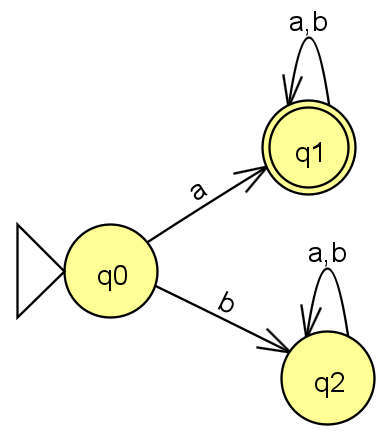
\includegraphics[width=0.2\textwidth]{../../../images/DFAs/ex1_q1.png}



% \vspace{3cm}
% \begin{flushleft}
% أرجو لكم وقتًا ممتعًا.

% الأستاذ محمود اغبارية.
% \end{flushleft}


% \end{document}


\ifwithsols
\title{حل ورقة تمرّن 19 - قسم 2 \\ مصفوفة كائنات + فئات مع مصفوفة}
\else
\title{ورقة تمرّن 19 - قسم 2 \\ مصفوفة كائنات + فئات مع مصفوفة}
\fi

\begin{document}

\maketitle
\thispagestyle{fancy}

\begin{enumerate}

%=============================================================
%--- سؤال 1 ---
%=============================================================
\item \textbf{مرآب سيارات}

اكتب فئة \textenglish{Parking} تمثل مرآباً للسيارات.
تتلقى العملية البناءة رقم المرآب (\textenglish{int}) وعدد أماكن الوقوف (\textenglish{int})،
وتُنشئ مصفوفة منطقية بنفس الحجم (القيمة الابتدائية \textenglish{false} تعني أن المكان فارغ).
على الفئة أن تدعم العمليات التالية:

\begin{itemize}
  \item \textenglish{ParkCar(int spotIndex) : bool} --
        تحجز المكان ذا الرقم \textenglish{spotIndex}،
        وتُعيد \textenglish{true} إذا نجحت العملية،
        أو \textenglish{false} إذا كان الرقم خارج النطاق أو المكان مشغولاً.

  \item \textenglish{RemoveCar(int spotIndex) : bool} --
        تُفرغ المكان ذا الرقم \textenglish{spotIndex}،
        وتُعيد \textenglish{true} إذا نجحت العملية،
        أو \textenglish{false} إذا كان الرقم خارج النطاق أو المكان فارغاً أصلاً.

  \item \textenglish{IsSpotFree(int spotIndex) : bool} --
        تتلقى رقم مكان وتُعيد \textenglish{true} إذا كان فارغاً،
        و\textenglish{false} إذا كان مشغولاً أو كان الرقم خارج النطاق.

  \item \textenglish{FreeSpots() : int} --
        تُعيد عدد الأماكن الفارغة حالياً.

  \item \textenglish{TotalSpots() : int} --
        تُعيد العدد الكلي للأماكن في المرآب.
\end{itemize}

اكتب في \textenglish{Main} كوداً ينشئ مرآباً برقم 5 وفيه 4 أماكن،
ثم يُوقف سيارات في الأماكن 0 و1 و3،
ثم يطبع عدد الأماكن الفارغة والكلية.

\ifwithsols
{\small
\begin{boxSolution}
\begin{english}
\begin{minted}{csharp}
class Parking
{
    private int    parkingId;
    private bool[] spots;

    public Parking(int parkingId, int spotsCount)
    {
        this.parkingId = parkingId;
        this.spots     = new bool[spotsCount]; // false = free
    }

    public bool ParkCar(int spotIndex)
    {
        if (spotIndex < 0 || spotIndex >= spots.Length
                          || spots[spotIndex])
            return false;
        spots[spotIndex] = true;
        return true;
    }

    public bool RemoveCar(int spotIndex)
    {
        if (spotIndex < 0 || spotIndex >= spots.Length
                          || !spots[spotIndex])
            return false;
        spots[spotIndex] = false;
        return true;
    }

    public bool IsSpotFree(int spotIndex)
    {
        if (spotIndex < 0 || spotIndex >= spots.Length)
            return false;
        return !spots[spotIndex];
    }
\end{minted}
\end{english}
\end{boxSolution}
\begin{boxSolution}
\begin{english}
\begin{minted}{csharp}
    public int FreeSpots()
    {
        int count = 0;
        for (int i = 0; i < spots.Length; i++)
            if (!spots[i]) count++;
        return count;
    }

    public int TotalSpots()
    {
        return spots.Length;
    }
}

public static void Main(string[] args)
{
    Parking p = new Parking(5, 4);
    p.ParkCar(0);
    p.ParkCar(1);
    p.ParkCar(3);
    Console.WriteLine("Free: "  + p.FreeSpots());   // 1
    Console.WriteLine("Total: " + p.TotalSpots());   // 4
}
\end{minted}
\end{english}
\end{boxSolution}
}
\fi
\clearpage

%=============================================================
%--- سؤال 2 ---
%=============================================================
\item \textbf{تقييم الطلاب}

اكتب فئة \textenglish{Classroom} تمثل صفاً دراسياً.
تتلقى العملية البناءة رقم الصف (\textenglish{int}) وعدد الطلاب (\textenglish{int})،
وتُنشئ مصفوفة من نوع \textenglish{double} بنفس الحجم وتُهيئ جميع قيمها بالصفر.
على الفئة أن تدعم العمليات التالية:

\begin{itemize}
  \item \textenglish{SetGrade(int studentIndex, double grade) : void} --
        تُسجّل العلامة \textenglish{grade} للطالب ذي الرقم \textenglish{studentIndex}.
        لا تأثير إذا كان الرقم خارج النطاق أو كانت العلامة خارج المجال $[0, 100]$.

  \item \textenglish{GetGrade(int studentIndex) : double} --
        تُعيد علامة الطالب ذي الرقم \textenglish{studentIndex}،
        أو $-1$ إذا كان الرقم خارج النطاق.

  \item \textenglish{Average() : double} --
        تُعيد معدل علامات جميع طلاب الصف.

  \item \textenglish{PassCount() : int} --
        تُعيد عدد الطلاب الذين علامتهم 60 أو أكثر.

  \item \textenglish{StudentCount() : int} --
        تُعيد العدد الكلي للطلاب في الصف.
\end{itemize}

اكتب في \textenglish{Main} كوداً ينشئ صفاً برقم 10 وفيه 5 طلاب،
يُسجّل لهم العلامات: 55، 70، 90، 45، 80،
ثم يطبع معدل الصف وعدد الناجحين.

\ifwithsols
{\small
\begin{boxSolution}
\begin{english}
\begin{minted}{csharp}
class Classroom
{
    private int      classId;
    private double[] grades;

    public Classroom(int classId, int studentCount)
    {
        this.classId = classId;
        this.grades  = new double[studentCount]; // 0.0 by default
    }

    public void SetGrade(int studentIndex, double grade)
    {
        if (studentIndex < 0 || studentIndex >= grades.Length
                             || grade < 0 || grade > 100)
            return;
        grades[studentIndex] = grade;
    }

    public double GetGrade(int studentIndex)
    {
        if (studentIndex < 0 || studentIndex >= grades.Length)
            return -1;
        return grades[studentIndex];
    }

    public double Average()
    {
        double sum = 0;
        for (int i = 0; i < grades.Length; i++)
            sum += grades[i];
        return sum / grades.Length;
    }
\end{minted}
\end{english}
\end{boxSolution}
\begin{boxSolution}
\begin{english}
\begin{minted}{csharp}
    public int PassCount()
    {
        int count = 0;
        for (int i = 0; i < grades.Length; i++)
            if (grades[i] >= 60) count++;
        return count;
    }

    public int StudentCount()
    {
        return grades.Length;
    }
}

public static void Main(string[] args)
{
    Classroom cls = new Classroom(10, 5);
    cls.SetGrade(0, 55);
    cls.SetGrade(1, 70);
    cls.SetGrade(2, 90);
    cls.SetGrade(3, 45);
    cls.SetGrade(4, 80);
    Console.WriteLine("Average: "    + cls.Average());    // 68.0
    Console.WriteLine("Passed: "     + cls.PassCount());  // 3
}
\end{minted}
\end{english}
\end{boxSolution}
}
\fi
\clearpage

%=============================================================
%--- سؤال 3 ---
%=============================================================
\item \textbf{مخزون صيدلية}

اكتب فئة \textenglish{Pharmacy} تمثل مخزون صيدلية.
تتلقى العملية البناءة اسم الصيدلية (\textenglish{string}) وعدد أنواع الأدوية (\textenglish{int})،
وتُنشئ مصفوفة من نوع \textenglish{int} بنفس الحجم وتُهيئ جميع قيمها بالصفر.
على الفئة أن تدعم العمليات التالية:

\begin{itemize}
  \item \textenglish{AddStock(int medicineIndex, int amount) : void} --
        تُضيف الكمية \textenglish{amount} إلى مخزون الدواء ذي الرقم \textenglish{medicineIndex}.
        لا تأثير إذا كان الرقم خارج النطاق أو كانت الكمية أصغر من 1.

  \item \textenglish{Dispense(int medicineIndex, int amount) : bool} --
        تُنقص الكمية \textenglish{amount} من مخزون الدواء ذي الرقم \textenglish{medicineIndex}،
        وتُعيد \textenglish{true} إذا نجحت العملية،
        أو \textenglish{false} إذا كان الرقم خارج النطاق أو الكمية المطلوبة غير متوفرة.

  \item \textenglish{GetStock(int medicineIndex) : int} --
        تُعيد كمية الدواء ذي الرقم \textenglish{medicineIndex}،
        أو $-1$ إذا كان الرقم خارج النطاق.

  \item \textenglish{OutOfStockCount() : int} --
        تُعيد عدد أنواع الأدوية التي نفدت (كميتها صفر).

  \item \textenglish{TotalUnits() : int} --
        تُعيد مجموع جميع الوحدات الموجودة في المخزون.
\end{itemize}

اكتب في \textenglish{Main} كوداً ينشئ صيدلية باسم \textenglish{"CityPharm"} وفيها 3 أنواع أدوية،
يُضيف 20 وحدة من الدواء 0، و15 من الدواء 2،
يصرف 8 وحدات من الدواء 0،
ثم يطبع عدد الأنواع التي نفدت وإجمالي الوحدات.

\ifwithsols
{\small
\begin{boxSolution}
\begin{english}
\begin{minted}{csharp}
class Pharmacy
{
    private string pharmacyName;
    private int[]  stock;

    public Pharmacy(string pharmacyName, int medicineCount)
    {
        this.pharmacyName = pharmacyName;
        this.stock        = new int[medicineCount]; // 0 by default
    }

    public void AddStock(int medicineIndex, int amount)
    {
        if (medicineIndex < 0 || medicineIndex >= stock.Length
                              || amount <= 0)
            return;
        stock[medicineIndex] += amount;
    }

    public bool Dispense(int medicineIndex, int amount)
    {
        if (medicineIndex < 0 || medicineIndex >= stock.Length
                              || amount <= 0
                              || stock[medicineIndex] < amount)
            return false;
        stock[medicineIndex] -= amount;
        return true;
    }

    public int GetStock(int medicineIndex)
    {
        if (medicineIndex < 0 || medicineIndex >= stock.Length)
            return -1;
        return stock[medicineIndex];
    }
\end{minted}
\end{english}
\end{boxSolution}
\begin{boxSolution}
\begin{english}
\begin{minted}{csharp}
    public int OutOfStockCount()
    {
        int count = 0;
        for (int i = 0; i < stock.Length; i++)
            if (stock[i] == 0) count++;
        return count;
    }

    public int TotalUnits()
    {
        int total = 0;
        for (int i = 0; i < stock.Length; i++)
            total += stock[i];
        return total;
    }
}

public static void Main(string[] args)
{
    Pharmacy ph = new Pharmacy("CityPharm", 3);
    ph.AddStock(0, 20);
    ph.AddStock(2, 15);
    ph.Dispense(0, 8);
    Console.WriteLine("Out of stock: " + ph.OutOfStockCount()); // 1
    Console.WriteLine("Total units: "  + ph.TotalUnits());      // 27
}
\end{minted}
\end{english}
\end{boxSolution}
}
\fi
\clearpage

%=============================================================
%--- سؤال 5 ---
%=============================================================
\item \textbf{نظام تصويت}

اكتب فئة \textenglish{Election} تمثل عملية انتخابية.
تتلقى العملية البناءة مصفوفة أسماء المرشحين \textenglish{string[]}.
الفئة تخزّن الأسماء وتُنشئ مصفوفة أصوات موازية لها مُهيأة بالصفر.
على الفئة أن تدعم العمليات التالية:

\begin{itemize}
  \item \textenglish{Vote(string name) : void} --
        تُضيف صوتاً واحداً للمرشح الذي اسمه \textenglish{name}.
        لا تأثير إذا لم يكن الاسم موجوداً في قائمة المرشحين.

  \item \textenglish{GetVotes(string name) : int} --
        تُعيد عدد أصوات المرشح الذي اسمه \textenglish{name}،
        أو $-1$ إذا لم يكن الاسم موجوداً.

  \item \textenglish{Winner() : string} --
        تُعيد اسم المرشح الحاصل على أعلى عدد من الأصوات.

  \item \textenglish{TotalVotes() : int} --
        تُعيد إجمالي عدد الأصوات التي أُدلي بها.
\end{itemize}

اكتب في \textenglish{Main} كوداً ينشئ انتخابات بين ثلاثة مرشحين:
\textenglish{"Ali"}، \textenglish{"Hanan"}، \textenglish{"Omar"}،
يُدلي بـ 4 أصوات لـ\textenglish{"Ali"}، و6 لـ\textenglish{"Hanan"}، و3 لـ\textenglish{"Omar"}،
ثم يطبع اسم الفائز وإجمالي الأصوات.

\ifwithsols
{\small
\begin{boxSolution}
\begin{english}
\begin{minted}{csharp}
class Election
{
    private string[] candidates;
    private int[]    votes;

    public Election(string[] candidates)
    {
        this.candidates = candidates;
        this.votes      = new int[candidates.Length]; // 0 by default
    }

    private int FindIndex(string name)
    {
        for (int i = 0; i < candidates.Length; i++)
            if (candidates[i] == name) return i;
        return -1;
    }

    public void Vote(string name)
    {
        int idx = FindIndex(name);
        if (idx != -1)
            votes[idx]++;
    }

    public int GetVotes(string name)
    {
        int idx = FindIndex(name);
        if (idx == -1) return -1;
        return votes[idx];
    }

    public string Winner()
    {
        int maxIdx = 0;
        for (int i = 1; i < votes.Length; i++)
            if (votes[i] > votes[maxIdx])
                maxIdx = i;
        return candidates[maxIdx];
    }
\end{minted}
\end{english}
\end{boxSolution}
\begin{boxSolution}
\begin{english}
\begin{minted}{csharp}
    public int TotalVotes()
    {
        int total = 0;
        for (int i = 0; i < votes.Length; i++)
            total += votes[i];
        return total;
    }
}

public static void Main(string[] args)
{
    string[]  names = { "Ali", "Hanan", "Omar" };
    Election  elec  = new Election(names);

    for (int i = 0; i < 4; i++) elec.Vote("Ali");
    for (int i = 0; i < 6; i++) elec.Vote("Hanan");
    for (int i = 0; i < 3; i++) elec.Vote("Omar");

    Console.WriteLine("Winner: "      + elec.Winner());      // Hanan
    Console.WriteLine("Total votes: " + elec.TotalVotes());  // 13
}
\end{minted}
\end{english}
\end{boxSolution}
}
\fi

\end{enumerate}

\vspace{1em}
\begin{flushleft}
أرجو لكم عملاً ممتعاً!

الأستاذ محمود اغبارية
\end{flushleft}

\end{document}
